\newpage
\fancyhead[C]{Thomas Turner}
\section{Return to Safety} \label{Return to Safety}

\subsection{Introduction and Philosophy}\label{sub_section:tgt_RTS_intro}
\gls{RTH} should always be used when possible as returning to the base is easiest and safest for ground operators. When the device experiences a significant probability of failure traditionally it carries out an emergency landing. However, in this specific operating environment emergency landing leaves the device stranded in a minefield where it cannot be retrieved. Therefore, a \gls{RTS} system is developed where it attempts to go to the nearest safe landing zone for retrieval minimising the probability of crashing in a dangerous environment and avoiding obstacles. This system should be practical, easy to use and supportive of those with disabilities.

\subsection{Cost Maps}
\subsubsection{Source data}
When considering \gls{RTS} it requires prior knowledge of the operating environment which is loaded into the drone using ground operators before flight. This is accomplished using bird's eye images of the operating areas and marking the obstructions, suspected mined regions, mildly dangerous regions, and safe landing regions, with corresponding \gls{GNSS} co-ordinates.
\paragraph{Satellite Images}
Where satellite images are available and accurate they are the easiest option. However, given the nature of environments effected by war, there may have been significant changes to the local environment since the last satellite image. Furthermore, seasonal changes can make satellite images less effective as trees may be less visible from winter images due to a lack of leaves.
\paragraph{Surveillance Images}
Standard consumer level drones can provide images with tagged \gls{GNSS} co-ordinates that can be used, however, this requires extra hardware and time to execute. Therefore, this should be avoided where satellite images are sufficient.

\subsubsection{Graphical User Interface}
\paragraph{Platform} 
The \gls{GUI} was considered from the start to maximise usability by untrained ground operators. I built the \gls{GUI} using a simple python script that takes an image path and uses hardware-independent click locations and keystrokes to operate. It then gives the output as a $.txt$ file with a standard format. This means that the process can be run on any local hardware available.
\paragraph{User interactions}
The user can click on a region to set it a colour representing the classification, there is also a separate mode that uses intensities not colours to support colour-blind ground operators. Semi-transparent shades are used so the base image can be seen through the shade of classification colour allows for a more natural filling experience. Furthermore, some utility functions including multi-zone filling, clicking on already classified regions to deselect and auto-filling regions were added to make the process easier and faster. The process from satellite image (from Google Earth), to cost map, to a flow map is shown in \ref{fig:cost map net}. The only information uploaded to the drone is \ref{fig:cost map flow} where the arrows denote where to go next and the circles denote where, if there, the device should land.

\subsubsection{Tessellated surfacing}
\paragraph{Hexagons} While squares and triangles are more widely used, they are worse than hexagons for this application as they are less intuitive. Travelling centre to centre on the diagonals of squares goes through a point of four intersection where the classification is undefined. Therefore if the user added two obstacles diagonally connected it is unknown if you could travel diagonally between them, this ambiguity creates issues that you do not face when using hexagons as while at the intersections the classifications are still undefined, when travelling centre to centre you never cross an intersection of more than two hexagons.
\paragraph{Mapping hexagons to \gls{GNSS}} \label{para:Mapping hexagons}
The two key methods of mapping from hexagons to Cartesians either uses two axial co-ordinates or using row and column values with an offset described in previous work\cite{MappingHexagons}. Once the converted into Cartesian form you multiply the values by the scaling factor to get offset from the origin. This is combined with the known location of the origin to generate the \gls{GNSS} tags for the centre of each hexagon.

\subsubsection{Efficient filling}
\paragraph{Auto-filling from Path Planning}
Having the ground user filling in both the path planning polygonal zones and the cost map is inefficient due to the shared information. Therefore, provided the images used are the same, the cost map automatically classifies hexagons with an obstacle listed within its bounds as an obstacle region. It also automatically classifies the region of interest as dangerous to land as it is a mined area. This reduces the number of zones required to be filled by the ground operator. 
\paragraph{Dynamic Zooming}
In complicated operating environments higher resolutions may be needed, however, often the major zones will remain the same. Therefore, the user will have two different views, the major view that is used to fill in large zones and the minor view that the user accesses in order to fill in smaller more detailed zones. 
\paragraph{Machine Learning Methods}
The cost map generating program not only records the final results but all of the ground operator times and clicks. This output file is sent to the development team, if the ground user has not disabled this functionality due to safety or privacy reasons. This will support future work to create new tools to reduce the time taken in combination with feedback.
\begin{figure}[htbp]
  \centering
  \begin{subfigure}[b]{0.32\textwidth}
    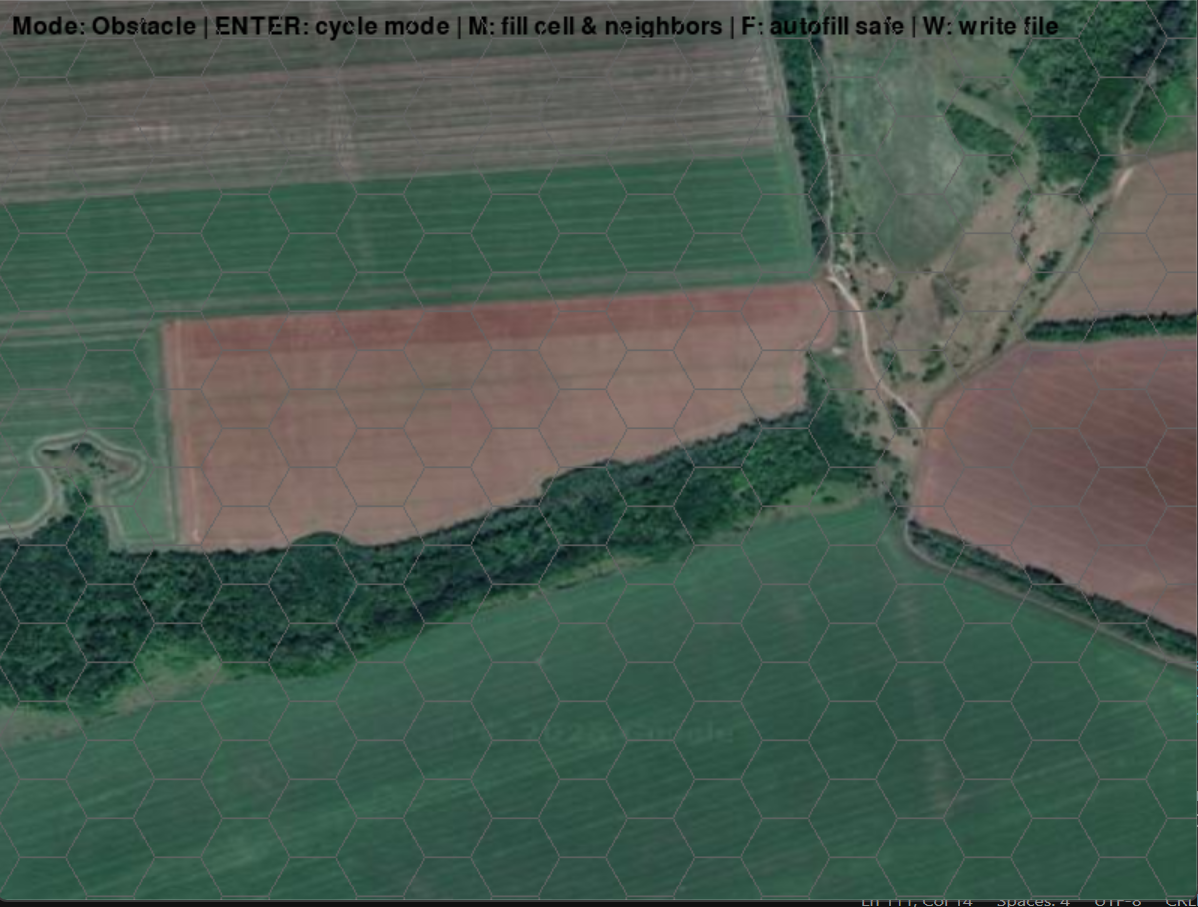
\includegraphics[width=\textwidth]{figs/Thomas/Return To Safety/50.19.27.N 36.55.32.E.png}
    \caption{Satellite Image}
    \label{fig:cost map satellite}
  \end{subfigure}
  \hfill
  \begin{subfigure}[b]{0.32\textwidth}
    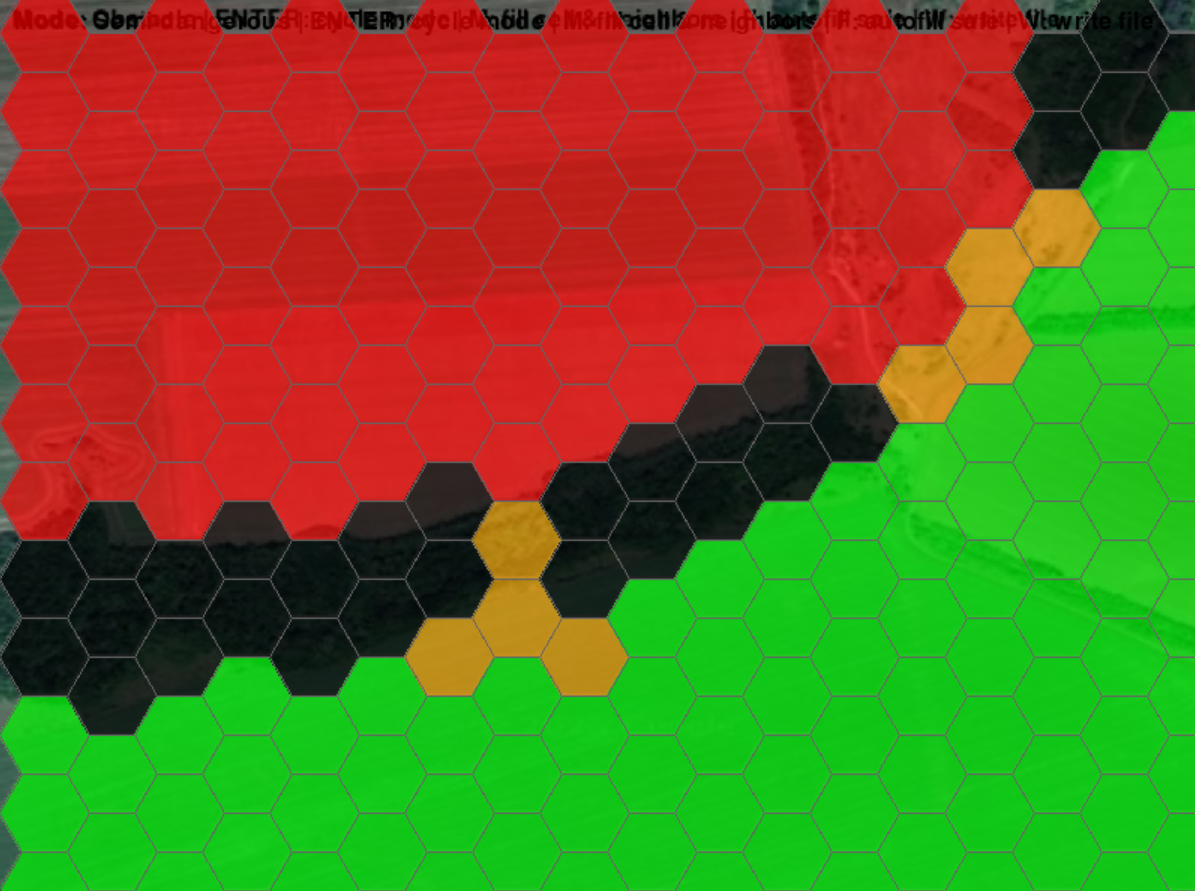
\includegraphics[width=\textwidth]{figs/Thomas/Return To Safety/50.19.27.N 36.55.32.E Cost.png}
    \caption{Cost Map}
    \label{fig:cost map cost}
  \end{subfigure}
  \hfill
  \begin{subfigure}[b]{0.32\textwidth}
    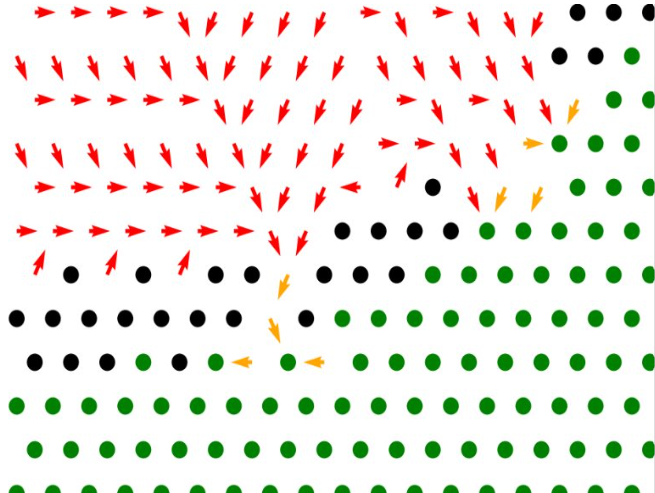
\includegraphics[width=\textwidth]{figs/Thomas/Return To Safety/50.19.27.N 36.55.32.E Flow.png}
    \caption{Flow Map}
    \label{fig:cost map flow}
  \end{subfigure}
  
  \caption{Geospatial analysis at coordinates 50.19.27.N 36.55.32.E}
  \label{fig:cost map net}
\end{figure}
\subsection{Fault Detection, Quantification and Control}\label{sub_section:tgt_fault_detection}

\subsubsection{State of Charge}\label{sub_sub_section:tgt_SOC}
\paragraph{Component Ageing}
Cell ageing and actuator ageing can cause inaccurate state of charge predictions. Therefore, the planned path may exceed the limit of the device leading to a state of charge fault and the necessity of \gls{RTH} if the state of charge is within 10\% of the predicted required state of charge required for \gls{RTH}. However, the state-vector telemetry recorded by the flight controller will be used to regularly inspect the cell performance and replace the cells or actuators if needed before failure.
\paragraph{Cell Failure}
\gls{Li-ion} batteries can have a thermal runaway. This is seen with a massive spike in temperature from the \gls{BMS} telemetry data and should lead to immediate landing and battery shutdown as it is a chain reaction effect that can cause excessive thermal damage\cite{LiONRunaway}.

\subsubsection{Actuator Fault}\label{sub_sub_section:tgt_actuator_fault}
\paragraph{Causes}
A loss of actuator effectiveness can be either from motor damage or propeller damage. The possible causes of motor damage specific to the operating environments include: wire damage, cooling blockages and dust or sand getting into the components. For propeller damage this could be from impacts, thermal effects or fatigue cracks.
\paragraph{Monitoring}
Consider motor effectiveness factors $\eta_i \in [0,1]$ as random walks. Using the \gls{RPM} telemetry, predicted thrust for each motor $T_{\text{pred},i} = \eta_i k_T \omega_i^2$ can be generated. This is used predict the acceleration using an \gls{EKF} observer, $\mathbf{a}_{prediction}$, of the device and then compare with IMU-measured acceleration,  $\mathbf{a}_{actual}$ to calculate the residual as shown in Equation \ref{eq:residual}. 
\begin{equation}\label{eq:residual}
    \mathbf{r}(t) = \mathbf{a}_{prediction}(t) - \mathbf{a}_{actual}(t)
\end{equation}
The model parameters $\eta_i$ can be approximated using \gls{EKF} updates. An \gls{EKF} is used due to its wide industry use and proven effectiveness and should be sufficient to handle the non-linearities of the model however, if is found to be insufficient a \gls{UKF} filter could be used instead \cite{WAN2000}.
\paragraph{Fault Detection}
If $\eta_i$ falls below $\eta_{\text{thresh}}$ failure is detected however this has a slow detection time for sudden faults. Given in the case of sudden faults \gls{RTS} should not be attempted due to the likelihood of crashing, a separate detection system is required to trigger emergency landing. The residual $\mathbf{r}(t)$ is shown in Equation \ref{eq:residual}, if there is a sudden spike in residual it is likely due to an extreme gust , a change in state dynamics or a sudden fault. In each case emergency landing should be attempted immediately. To detect this spike with changing residual dynamics which can be caused by increased wind or sensor drift, the mean and covariance of $\mathbf{r(t)}$ are found as shown in Equations \ref{eq:residual_mean} and \ref{eq:residual_cov} where  $\mathbf{\tilde{r}}(t) = \boldsymbol{\tilde{r}}(t) - \boldsymbol{\mu_r}(t)$, and $\alpha \in [0,1)$ is the forgetting factor that will be tuned during testing \cite{roberts1959}.
\begin{equation}\label{eq:residual_mean}
     \boldsymbol{\mu_r}(t) = \alpha \boldsymbol{\mu_r}(t-1) + (1 - \alpha) \mathbf{r}(t)
\end{equation}
\begin{equation}\label{eq:residual_cov}
    \boldsymbol{\Sigma_r}(t) = \alpha \boldsymbol{\Sigma_r}(t-1) + (1 - \alpha) \boldsymbol{\tilde{r}}(t)\boldsymbol{\tilde{r}}(t)^T
\end{equation}
The acceptance range is then set using Equation \ref{eq:bounds} with sensitivity $k$ that can be tuned during testing. Then if $\mathbf{r(t)}$ has a value outside the acceptable region a fault is triggered \cite{Perry2010}. This provides a computationally lightweight algorithm well suited for real-time embedded application that automatically adjusts the detection bounds based uppon the characteristics of the sensors. This is especially important in \gls{UAV}s due to the gyroscopic drift and exposure to gusty winds that can cause false positives with fixed bounds.
\begin{equation}\label{eq:bounds}
    C_{\text{acceptance}}(t) = \boldsymbol{\mu_r}(t) \pm k \sqrt{\text{diag}(\boldsymbol{\Sigma_r}(t))}
\end{equation}
\paragraph{Reconfiguration}
For path planning as discussed in Section \ref{sub_sub_section:tgt_weather_failure} we need known characteristics of the device, specifically its travel speed and maximum wind speed rejection. Therefore, pre-computed control gains are calculated for different intervals of $\eta$, simulated and then tested with hardware-in-the-loop using fault injections. These controllers are preloaded into the device. These controllers are more robust to parameters and less aggressive then during typical operation to minimise the risk of actuator saturation, instability due to parameter inaccuracy and further damage to actuators. In order for the control behaviour to remain applicable with differing model parameters the motor control signals, $\mathbf{E}$, are scaled as shown in Equation \ref{eq:adj_thrust} where $\mathbf{N} = \text{diag}(\eta_1, \dots,\eta_4)$.
\begin{equation}\label{eq:adj_thrust}
    \mathbf{E}_{\text{adjusted}} = \mathbf{N}^{-1}\times \mathbf{E}_{\text{control}}, 
\end{equation}
If any $\eta_i$ falls below a threshold $\eta_{\text{thresh}}$ for each controller it will be transferred to different control gains and if any $\eta_i$ falls below $\eta_{\text{critical}}$ it will trigger emergency landing. To ensure transitions between controllers is smooth, the transition step should be simulated and tested with hardware before deployment. If this proves ineffective due to saturation of the damaged actuators, constrained quadratic programming can be used \cite{JOHANSEN2013} to distribute thrust to the stronger motors.

\begin{comment}
Furthermore, using static thresholds can lead to false positives when performing aggressive manoeuvres or in gusty conditions. This can be mitigated using statistical methods as explored in \cite{REF} but given that the device follows smooth paths and does not fly in extreme weather this mitigation is unnecessary.
\paragraph{Control Strategy}
The simplest solution is to tune the output signals from the controller until the thrust of the actuator matches the expected value. This allows the control loop to be unchanged, abstracting from the physical effects. However, the actuator will saturate at a lower thrust value meaning the control loop will not perform as expected and can lead to failure in typically non-failure states. By increasing the output on the actuator it will likely cause the current defect to degenerate as the loads increase on the damaged actuator. Therefore, a gain scheduling approach is used with a selection of less aggressive controller gains to match different tuning magnitudes. As tuning magnitude increases, the controller should be less aggressive so that the thrust demands reduce. However, this means that the controller cannot tolerate disturbances of the same magnitude. 

    \paragraph{Detection}
Leveraging the \gls{ESC} telemetry values of Voltage (V), Current (I) and Rotational Speed (RPM) in addition to the the \gls{IMU} data a Thrust/Power model of each motor is built.
For each control signal the predicted thrust values are used in combination to the inertial properties of the device to create an acceleration prediction vector $\mathbf{a}_{prediction}$. The actual acceleration,  $\mathbf{a}_{actual}$, is recorded using the \gls{IMU}.
\begin{equation}\label{eq:residual}
    \mathbf{r}(t) = \mathbf{a}_{prediction}(t) - \mathbf{a}_{actual}(t)
\end{equation}
The residual $\mathbf{r}(t)$ is shown in Equation \ref{eq:residual} and if the autocorrelation of $\mathbf{r}(t)$ over a sustained period it shows that there is a rotor fault or a change in the dynamics of the device. 
\paragraph{Quantification}


\paragraph{Isolation}
This means that the system is vulnerable to multiple actuator faults as all others are assumed healthy. There are methods that can address this at the cost of extra complexity \cite{ZHANG2008}. Given that the probability of simultaneous partial faults is low these are not necessary for this application, however, common mode failures could be possible for example if in sand storm you would expect multiple faults.


\end{comment}

\subsection{Emergency Path Planning}\label{sub_section:tgt_path_planning}

\subsubsection{Cost Function}\label{sub_sub_section:tgt_cost_function}
The key objective is to reduce the downtime and cost of operation of the drone. This means both the cost of damage to the drone through crashing and the difficulty of retrieval need consideration. Considering the centre of each hexagon in the cost map as a node and modelling the probability of surviving half of a node node traversal between adjacent nodes as constant, $p$, the cost function of any path of length $D$ is shown in \ref{eq:cost function}. The specific $c_{crashing}$ and $c_{landing}$ can be defined by the ground operators for each classification. The ones used in testing are shown in \ref{tab:cost_values}.
\begin{equation}\label{eq:cost function}
    E(x) 
    = \sum_{n=1}^{D-1} c_{crashing}\bigl(x_n\bigr)\, (1-p) \,p^n 
    \;+\; c_{landing}\bigl(x_D\bigr)\, p^D
\end{equation}
\begin{table}[h]
    \centering
    \begin{tabular}{|c|c|c|c|c|}
    \hline
         \textbf{} & \textbf{Safe} & \textbf{Semi-Dangerous} & \textbf{Dangerous} & \textbf{Obstacle} \\
         \hline
         \textbf{$c_{landing}$} & 0 & 1 & 10 & 100 \\
         \textbf{$c_{crashing}$} & 10 & 10 & 100 & 1000\\
         \hline
    \end{tabular}
    \caption{Testing Costs}
    \label{tab:cost_values}
\end{table}

\subsubsection{Weather induced failure}\label{sub_sub_section:tgt_weather_failure}
\paragraph{Cause}
When a gust of wind exceeds the control capabilities of the drone it will cause an extreme disturbance and likely failure resulting in a crash. This is especially important to consider when their is an actuator fault due to the less aggressive control strategies deployed meaning that the maximum rejected gust becomes lower in magnitude and therefore more likely to occur. 
\paragraph{Gust Modelling}
Using forecasts and modelling as discussed in Section \ref{gust} we can model the probability that a gust exceeds the known maximum rejection gust speed for the current control gains per second, $\lambda$. From this we can calculate $p$ using Equation \ref{eq:p_calc}. The exact methods used to find $\lambda$ are an area of future work.
\begin{equation}\label{eq:p_calc}
    p = (1-\lambda)^{\frac{distance}{speed}}
\end{equation}

\subsubsection{Search Algorithms}\label{sub_sub_section:tgt_search}
\begin{algorithm}
\caption{Exhaustive Search}
\label{alg:search}
\begin{algorithmic}[1]
    \For{each Node $n$}
        \State $\textit{min\_cost} \gets \infty$
        \State $n.path\_cost$ = \Call{search}{$n$, $p$, $1$, $0$, $depth$, $\textit{min\_cost}$}
    \EndFor
    
    \Function{search}{$n$, $p$, $p\_alive$, $cost$, $depth$, \textbf{ref} $\textit{min\_cost}$}
        \State $\textit{current\_cost} \gets cost + p\_alive \cdot n.\textit{landing\_cost}$
        \If{$\textit{current\_cost} < \textit{min\_cost}$}
            \State $\textit{min\_cost} \gets \textit{current\_cost}$
        \EndIf
        \If{$depth = 0$ $\mathbf{or}$ $n.\textit{landing\_cost} = 0$ $\mathbf{or}$ $cost > \textit{min\_cost}$}
            \State \Return
        \EndIf
        \For{each $\textit{neighbour}$ in $n.\textit{neighbours}$}
            \State $p\_alive\_next \gets p\_alive \cdot p$
            \State $cost\_next \gets cost + p\_alive \cdot (1 - p) \cdot n.\textit{crashing\_cost}$
            \State \Call{search}{$\textit{neighbour}$, $p$, $p\_alive\_next$, $cost\_next$, $depth - 1$, $\textit{min\_cost}$}
        \EndFor
    \EndFunction
\end{algorithmic}
\end{algorithm}
\begin{algorithm}
    \caption{Smooth}
    \label{alg:flow}
\begin{algorithmic}[1]
    \While{not $Converged$}
        \State $Converged \gets TRUE$
        \For{each Node $n$}
            \For{each \textit{neighbour} in $n.\textit{neighbours}$}
                \State $\textit{movement\_cost} \gets n.\textit{crashing\_cost} \cdot \frac{1 - p}{2} +  \textit{neighbour}.\textit{crashing\_cost} \cdot \frac{p(1 - p)}{2}$
                \State $\textit{total\_cost} \gets \textit{movement\_cost} + p \cdot \textit{neighbour.path\_cost}$
                \If{$\textit{total\_cost} < n.\textit{path\_cost}$}
                    \State $n.\textit{path\_cost} \gets \textit{total\_cost}$
                    \State $Converged \gets FALSE$
                \EndIf
            \EndFor
        \EndFor
    \EndWhile
\end{algorithmic}
\end{algorithm}
\paragraph{Exhaustive Search}
The simplest algorithm is the recursive function shown in Algorithm \ref{alg:search}. There are steps taken to increase the efficiency, including pruning lines that already exceed the minimum cost as the cost is monotonic increasing and automatically terminating lines when they can land safely. However, the worst case time complexity remains $O(|V|6^{depth})$ as each node has 6 neighbours that get called recursively. To get guaranteed correct results it would require searching all paths as long as $|V|$ as costs cannot fall below 0 so it is never advantageous to revisit a node. Therefore, the worst case complexity for guaranteed optimal paths is $O(|V|6^{|V|})$. This is not usable for practical applications, therefore it requires a compromise to depth of search, no longer getting optimal path results.
\paragraph{Bellman-Ford}
To combat the issues with Algorithm \ref{alg:search}, I developed Algorithm \ref{alg:flow}. This algorithm smooths out the differences in path cost between neighbouring nodes following the Bellman-Ford algorithm. This guarantees correct answers when the nodes have fully converged. Bellman-Ford algorithms have a time complexity of $O(|E|\times |V|)$. In dense graphs this becomes  $O(|V|^3)$ however, we know $|E| \leq |V| \times 7$ as we are using hexagons can have an edge to 6 neighbours and a self edge indicating landing. Therefore the actual complexity is $O(|V|^2)$\cite{cormen2009}. This means it is practical to generate guaranteed optimal path results.

\subsubsection{Real-time application}\label{sub_sub_section:tgt_real_time}
\paragraph{Pre-Compute}
Carrying out memory and time complex operations on real-time hardware should always be avoided as operations require specific timings for optimal use. If all the values are pre-computed and uploaded to the device, the time and memory complexity becomes $O(1)$ which supports precise, timed operations. Within the path planning workflow, as much as possible should be pre-computed and simply accessed, however, if any algorithms are deployed they should be $O(1)$.
\paragraph{$p$ ranges}
While the value of $p$ can take any value between 0 and 1, there can be only 7 outputs for the next best move (going to each of the 6 neighbours or landing). Therefore, instead of creating a specific map for a specific value of $p$ on the flight controller you can pre-compute all the ranges of $p$ that would cause each of these outcomes. Then the device selects the option corresponding to its current $p$ value.
\paragraph{Deployment}
For a deployed algorithm consistent timings and a minimal memory footprint are essential. The algorithm \ref{alg:threshold} is used to select the next action based on the value of $p$ and the node $p$ ranges.
\begin{algorithm}[htbp]
  \caption{Threshold-Based Action Selection}
  \label{alg:threshold}
  \begin{algorithmic}[1]
    \Require Sorted threshold array \(\mathcal{P} = [p_1, p_2, \dots, p_6]\), associated actions \(\mathcal{A} = [a_1, a_2, \dots, a_6]\), input probability \(p\), default landing action \(a_{\textit{land}}\)
    \Ensure Selected action \(a\), GNSS coordinates \((\textit{lat}, \textit{lon})\)
    
    \State \(a \gets a_{\textit{land}}\) \Comment{Default to landing}
    \For{\(i = 1\) to \(n\)}
      \If{\(p < p_i\)}
        \State \(a \gets a_i\)
        \State \textbf{break}
      \EndIf
    \EndFor
    
    \State \((\textit{row}, \textit{col}) \gets \textit{GridCoordinates}(a)\)
    \State \((\textit{lat}, \textit{lon}) \gets \Call{ConvertToGNSS}{\textit{row}, \textit{col}}\)
    
    \State \Return \((a, \textit{lat}, \textit{lon})\)
  \end{algorithmic}
\end{algorithm}
\paragraph{Memory Management}
The memory on the \gls{MCU}s consists of Flash and \gls{SRAM}. Flash is static memory that has to be pre-loaded onto the board before each run whereas \gls{SRAM} is volatile but has faster access times. Therefore, waypoints, maps and gains are loaded into \gls{RAM} from the preset values in Flash before a flight. In addition, the flight controller's \gls{MCU} has \gls{ITCM} configured \gls{RAM} and \gls{DTCM} configured \gls{RAM}. \gls{DTCM} and \gls{ITCM} allow for precise timings when accessing data and instructions respectively and should therefore be used for looped processes including control loops and heading calculations. Whereas, for less timing critical actions or varying time operations such as actuator tests the regular \gls{SRAM} can be used. For the \gls{GNSS} module \gls{MCU} there is just Flash and \gls{SRAM} however, as it is a less complex operational loop this is sufficient. 
\begin{table}[h]
\centering
\begin{tabular}{ccccc} 
\toprule
\textbf{Device}&\textbf{Flash}&\textbf{SRAM}&\textbf{DTCM}&\textbf{ITCM}\\
 & (megabytes)& (kilobytes)& (kilobytes)& (kilobytes)\\
\midrule
STM32H743VGT6\tablefootnote{\url{https://www.st.com/en/microcontrollers-microprocessors/stm32h743vg.html}}&1&1000&128&64\\
MSPM0G3506SRHBR\tablefootnote{\url{https://www.ti.com/product/MSPM0G3506/part-details/MSPM0G3506SRHBR}}&0.128&64&-&-\\
\bottomrule
\end{tabular}
\caption{MCU Memory}
\label{tab:MCU_memory}
\end{table}

\paragraph{Memory Reduced Nodes}
Using a C implementation as shown in Listing \ref{lst:node} it requires 56 bytes per node, therefore, for a 256 node map it requires 14.336 kilobytes of \gls{RAM}. This puts significant resolution limitations on the map. Therefore, the map should be stored in custom data structures that contain only as many bits as required. By using an indexed node array instead of pointers, 12 bit indexes can be used supporting 4096 nodes and 8 bits for probability values is sufficient. Lastly, the index of the node can be used to derive its location removing the relative values. This structure is shown in Listing \ref{lst:reducednode} and with the above values and using guaranteed optimal number of thresholds and actions of 6 results in 16.5 bytes per node. However, the major drawback is that when moving away from from standard C data types bespoke bit operations are required increasing the development difficulty. 
\paragraph{Stop-Go Method}
The nature of the problem can be exploited using the strategy of the map having one option for the next move that above a probability threshold it goes to, and below that threshold it lands. This means that only one action and one threshold in the \ref{lst:reducednode} reduced node structure is needed resulting in a memory intensity of 4 bytes per node.
\begin{lstlisting}[caption={Implementated Node Structure},label={lst:node}]
struct Node {
    float rel_long, rel_lat;  // relative longitude and lattidue to reference point
    float p_values[6];        // Probability thresholds
    Node* actions[6];         // Points to the next node
};
\end{lstlisting}
\begin{lstlisting}[caption={Node Structure},label={lst:reducednode}]
struct Node {
    idx;           // Current Index Position
    p_values[];    // Probability thresholds
    actions[];     // Indexes of the next node
};
\end{lstlisting}

\paragraph{Testing}
Using 10 random satellite images from the Kharkiv region, 256 node cost maps were generated including visible obstacles and assumed regions of interest. Each trail consisted of starting at each node in the region of interest and finding the actual cost, using the values given in Table \ref{tab:cost_values}, experienced following maps generated by each nodal structure for a specified value of $p$. 20 trials were run between $p$ values 0.01 and 0.99 with intervals of 0.01 and the aggregate average performances between Stop-Go, Reduced and Implemented nodes were all within 0.01\% showing equivalent performance of each nodal structure over the dataset. However, the Stop-Go method can no longer guarantee optimal results leaving them vulnerable to unforeseen situations and varying cost functions. Therefore, the reduced node given in Listing \ref{lst:reducednode} should be implemented unless there are significant memory requirements.



\subsection{Conclusion}
The \gls{GUI} is easy and quick to use for untrained ground operators and supports the colour-blind. The path planning algorithm supports pre-computation that enables the device to operate \gls{RTS} with $O(1)$ memory and time complexity supporting real-time deployment. Finally, the system is built to be flexible with improvements in mind by setting up the data collection architecture to enable to the system to improve with use. 